%!TEX root = ../../Heun_Dale_Haney_A_dynamic_approach_to_input_output_modeling.tex
%%%%%%%%%%%%%%%%%%%%% chapter.tex %%%%%%%%%%%%%%%%%%%%%%%%%%%%%%%%%
%
% sample chapter
%
% Use this file as a template for your own input.
%
%%%%%%%%%%%%%%%%%%%%%%%% Springer-Verlag %%%%%%%%%%%%%%%%%%%%%%%%%%
%\motto{Use the template \emph{chapter.tex} to style the various elements of your chapter content.}
\motto{Where there is no reliable accounting 
and therefore no competent knowledge
of the economic and ecological effects of our lives,
we cannot live lives that are economically
and ecologically responsible. 
It is futile to plead and protest and lobby 
in favor of public ecological responsibility while, 
in virtually every act of our private lives, 
we endorse and support an economic system 
that is by intention, 
and perhaps by necessity, 
ecologically irresponsible.~\emph{\cite[p.~26]{Berry1998}}

\hfill---\emph{Wendell Berry}}


\chapter{Introduction}
% use \chaptermark{}
% to alter or adjust the chapter heading in the running head
\chaptermark{Introduction}
% Always give a unique label
\label{chap:intro}

\abstract*{[NEED TO ADD ABSTRACT HERE]}

%% \abstract{Each chapter should be preceded by an abstract (10--15 lines long) that summarizes the content. The abstract will appear \textit{online} at \url{www.SpringerLink.com} and be available with unrestricted access. This allows unregistered users to read the abstract as a teaser for the complete chapter. As a general rule the abstracts will not appear in the printed version of your book unless it is the style of your particular book or that of the series to which your book belongs.\newline\indent
%% Please use the 'starred' version of the new Springer \texttt{abstract} command for typesetting the text of the online abstracts (cf. source file of this chapter template \texttt{abstract}) and include them with the source files of your manuscript. Use the plain \texttt{abstract} command if the abstract is also to appear in the printed version of the book.}

%% Use the template \emph{chapter.tex} together with the Springer document class SVMono (monograph-type books) or SVMult (edited books) to style the various elements of your chapter content in the Springer layout.

%DISCUSSION POINTS
%\begin{itemize}
%	% \item{Is `society' the best word – `final consumption?'}
%	%	\item{Do we use energy circuit language?}
%	% \item{For economists, capital is only in the productive sector, 
%	%$\dot{K}_{i1}$ flows would be `consumer durables'}
%	\item{Housing is `residential capital'}
%\end{itemize}

This book is primarily about accounting and change. 
It is born out of a belief that our economies are in constant flux;
changing dynamically in the short-term with human behavior 
and evolving over longer time frames to new inventions and
pressures from outside.
Real-world systems are messy and chaotic.
They do not march neatly from one stage to the next 
in an orderly fashion.

This is also a book about models and metaphors.
The real world influences the mental models 
by which we come to frame the world and 
the metaphors we use to describe it.
We perceive the world by the data we collect.
We interpret the real world through our models
which are influenced by our metaphors.
The things that we account 
(and by extension those things we leave out)
indirectly influence our behavior.
These models then mold the real world by shaping our
interactions with it.
Feedback loop - models to accounting to behavior to metaphors to models.
Our accounting systems are inextricably linked 
with our models inform us what is important to measure.
In order to better understand the complex dynamics 
of real-world economies, 
our model economies
(the ones that exist in our minds)
need to be able to cope with rapid transience,
not just ordered stability.




%%%%%%%%%% Motivation	%%%%%%%%%%
\section{Motivation}
\label{sec:motivation}
%%%%%%%%%%

\begin{quotation}
The world needs another industrial revolution 
\emph{in which our sources of energy are affordable, 
accessible and sustainable. 
Energy efficiency and conservation, 
as well as decarbonizing our energy sources, 
are essential to this revolution.}~\cite[p.~294]{Chu2012}\\
\begin{flushright}
---Steven Chu, US Secretary for Energy
\end{flushright}
\end{quotation}


\begin{quotation}
\emph{In developed economies we live the good life for now –-
with an amazing level of comfort and interest 
created by our astonishing ability to 
make and transform materials. 
We've really only done this at scale in the past 150 years, 
in which time our use of engineered materials has rocketed, 
literally. 
However, if we have some concern about `sustainability' 
we need to anticipate what effects our use might have 
on future generations –-
and we're getting some clear indicators that there's a 
problem.}~\cite[p.~3]{allwood2012sustainable}
\begin{flushright}
---Julian Allwood
\end{flushright}
\end{quotation}

The original motivation for writing this book
came from a belief that our global economy is
facing a necessary transition and that in order
to adequately manage this transition,
we need to better understand our economies.
What transition are we facing?The twin dictates of climate change and 
sustainable development require a transition to a
low-emission energy system based on 
non-depletable resources. 
Given that our energy system currently runs
primarily on non-renewable resources (fossil fuels),
we essentially need to rebuild our entire energy
system.

Furthermore,
our economies are founded on a fundamental principle;
\emph{the moral imperative of economic growth}.~\cite{Daly1995}
Growth in production and consumption of goods and services
entails the encroachment of the human economy into the
biosphere on which it is dependent.
One more table means one less tree.
As we increase the scale of the economy,
we increase the environmental impact of all of our actions.
There is good reason to believe that the earth 
is running low on its ability to handle more growth in
human impact.\cite{UNMEA2005}

In the face of such fears,
the hopeful vision of ``dematerialization'' 
has appeared (materialized).~\cite{Bernardini1993, Wernick1996, Cleveland1998}
We can continue to grow our economies
while reducing our impact on the environment.
Our increasing knowledge and use of technology will
allow us to reduce the material consumption of 
our goods and services.
In order to achieve such a dematerialization 
will require changing the structure of our economies.

The driving motivation behind this book is 
an attempt to understand
the structural elements of our economies,
not just the flows;
to understand the circulatory system,
not just the blood.
It is only by understanding this structure that we can 
begin to understand how our economies change.
And it is only by understanding how our economies change
that we can understand how best to manage this necessary
transition.

%%%%%%%%%%	Model-metaphors	%%%%%%%%%%
\section{Models-metaphors for the economy}
\label{sec:metaphors}
%%%%%%%%%%

In its most basic form,
a model is any ``simplified representation 
of reality''.~\cite[p.~105]{Meadows1992}
Our concept of ``reality'' is a vastly simplified
mental model of the real world.
These mental representations are vital to theory
consruction in science, 
since they mediate between 
human cognition and phenomena.
The power of our models lies in explaining
some aspect of our universe.
The appeal of these explanations lies in their
relative simplicity.
Interwoven with this simplification are the analogies
or metaphors we use to describe or communicate
our models.
Metaphors contextualize new models and theory
with reference to familiar settings and events,
often from everyday experience.
The archetypal (classic?) example is classical
physics representation of the ``clockwork''
universe.
Our models (and subsequently the metaphors we
use to talk about them) guide our actions
and interactions with the real world.
Firstly, a model tells us what aspects of the world
are important to value 
(in the literal sense of making measurements),
 and also, by extension, 
 which parts of the world (literally) have no value.
This evaluative procedure has a deeper normative
consequence.
That the aspects of the world to which our model places
value are valuable and that those 
that have no value are worthless.
Thus metaphors inform our thinking about the
real world,
but consequently,
they may also constrain our ability to
frame reality.
We interact with reality in the manner 
with which we interact with the objects of our
metaphors.
We mistake the model-metaphor for reality.
Classical physics tells us the universe is
\emph{like} clockwork, 
hence we begin to interact with it 
as if it \emph{really were} clockwork.

In the next sections we will explore some of the
models and metaphors associated with different
views of the economy.

\begin{svgraybox}
{\large \textbf{A primer on system theory:}}
\\\\
Some concepts of system theory will aid the discussion
in the rest of this chapter.
Those familiar with thermodynamics or general system
theory may skip over the following sections.
Systems are generally characterized within three
distinct categories: 
isolated, closed and open systems.
\\\\
\noindent{\large \textbf{\emph{Isolated systems}}}\\\\
Isolated systems (Figure~\ref{fig:systems}A)
are disconnected from their environment
such that neither energy nor material crosses the
boundary of the system.
Inside the boundary,
materials and energy may be exchanged
between element of the system.
The concept of an isolated system is used regularly
in thermodynamics to represent an ideal,
perfectly insulated container with no heat flow 
to or from the environment.
Within the universe no systems are truly isolated,
since all must interact with their environment
to at least some degree.
The universe itself may be an example of an 
isolated system.
\\\\
\noindent{\large \textbf{\emph{Closed systems}}}
\\\\
A closed system (Figure~\ref{fig:systems}B)
can exchange energy, but not materials,
with its environment.
The earth is often considered to be a closed system.
There is little exchange of material---some meteorites
and loss of atmospheric gases---but a large incoming
flow of solar radiation balanced (according to the 
Law of Conservation of Energy) by dissipation of (infra-red) radiation.
The incoming radiation, at $\approx$ 5000K, is of much
higher quality than the thermal radiation, which leaves at a 
temperature of $\approx$ 300K.
This degradation in energy quality drives practically
all of the biological processes on Earth.
\\\\ 
\noindent{\large \textbf{\emph{Open systems}}}
\\\\
Open systems (Figure~\ref{fig:systems}C),
as the name suggests, are open
to flows of both energy and materials.
The biosphere is a good example of an open system.
It exchanges energy and materials with the other systems
(atmosphere, hydrosphere, lithosphere)~\cite{Johnson1997}
of the earth, of which it is a subset.
\\\\
\noindent{\large \textbf{\emph{Feedback and non-linearity}}}
\\\\
Feedback occurs when elements of a system interact so as
to reinforce or diminish some property of the system.
For example, if the rate of growth of a population
is dependent on the size of that population.
If the rate of growth \emph{increases} as population increases,
we say that the feedback is \emph{positive} or \emph{reinforcing}.
If the rate of growth \emph{decreases} as population increases,
we say that the feedback is \emph{negative} or \emph{correcting}.
Often feedback systems involve some method of control or 
intentional regulation,
as in self-regulating systems.
Systems containing feedback loops will often display
non-linear or even chaotic behavior. 
Such systems may also display \emph{resilience},
even in the face of large changes in external conditions.
\\\\
\noindent{\large \textbf{\emph{Self-regulating systems}}}
\\\\
Organisms are open systems.
They maintain their internal structure by taking in
high quality energy and materials from 
and expending low quality to their
environment. 
This maintenance requires an ability to regulate
internal conditions,
such as temperature or chemical composition, 
known as \emph{self-regulation}.
Self-regulation relies on feedback among system elements.
Non-living systems may also display self-regulating behavior.
\\\\
\noindent{\large \textbf{\emph{Emergence and hierarchy}}}
\\\\
Due to the non-linear nature and complexity of natural systems,
new \emph{emergent} properties arise which cannot
be explained solely in terms of the properties 
of the elements of which
the system is composed.
An obvious example is the emergence of life from
large molecular structures.
Because the properties of the system are
\emph{irreducible} to properties of the system elements,
we may envision a hierarchy of nested systems.
Boulding~\cite{Boulding1956} classifies a number
of system levels (outlined in Table~\ref{tab:hierarchy})
ranging from simple \emph{structures} (atoms, bridges) up
to \emph{transcendental systems} such as religion.
\\\\
\noindent{\large \textbf{\emph{Self-organizing systems}}}
\\\\
Self-organization involves spontaneous increase in complexity
of the internal structure of a system,
normally observed in systems far from equilibrium.
Examples are the formation of convection cells 
in heated fluids~\cite{Benard1901}
The self-organizing behavior is an
emergent property of the system;
it cannot be explained in terms of properties
of the system elements.
\end{svgraybox}

\begin{figure}
\label{fig:systems}
\begin{center}
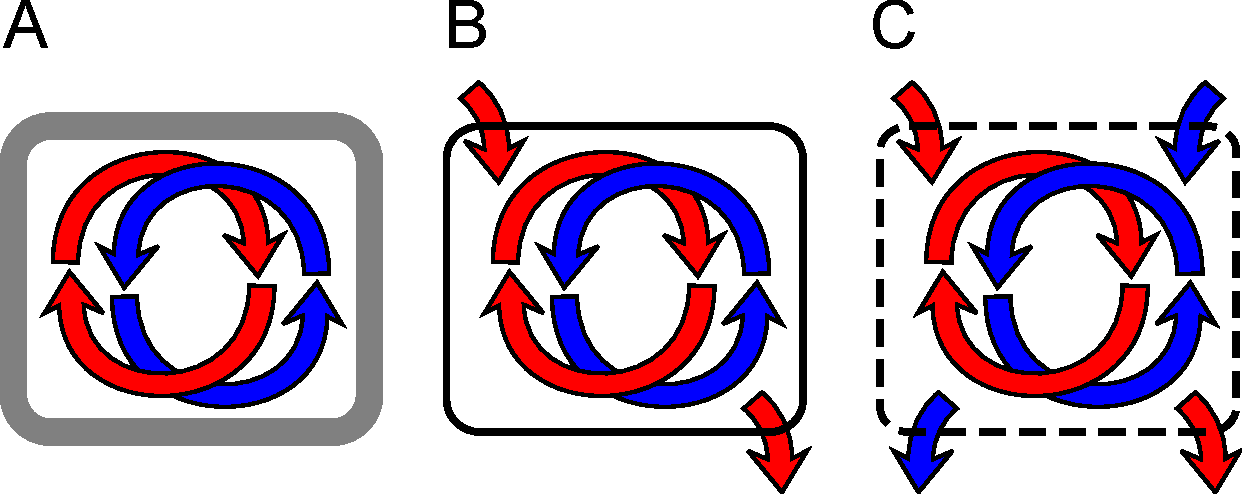
\includegraphics[width=\linewidth]{Part_0/Chapter_Introduction/images/systems.pdf} 
\end{center}
\caption[Isolated, closed and open systems]{Isolated (A), 
closed (B) and open (C) systems}
\end{figure}

\begin{table}
\caption[Hierarchy of systems]{Hierarchy of systems~\cite{Boulding1956}}
\begin{tabular}{r@{\hspace{1em}}l@{\hspace{1em}}l@{\hspace{1em}}l}
\toprule
\textbf{Level}	& \textbf{Description}	&	\textbf{Characteristic}	&	\textbf{Examples}	\\
\midrule
1	&	Structures	&	Static, spatial frameworks &	Atom, crystal, bridge	\\
2 & Clockworks & Predetermined motion	& Solar system, clocks, machines\\
3 & Control & Closed-loop feedback control mechanism & Heater with thermostat \\
4 & Open systems & Structurally self-maintaining	& Cells	\\
5	& Genetic systems & Community of cells & Plants	\\
6	& Animals	&	Nervous system, self-awareness & Birds and beasts	\\
7 & Humans & Self-consciousness, knowledge,
language & Human beings	\\
8 & Socio-cultural systems	&	Roles, values, communication &	Family, community, society	\\
9	&	Transcendental systems	&	Beyond our knowledge	&	Religion	\\
\bottomrule
\end{tabular}
\label{tab:hierarchy}
\end{table}

%%%%%%%%%%	Mechanistic	%%%%%%%%%%
\subsection{Traditional mechanistic view of economy}
\label{sec:mechanistic}
%%%%%%%%%%

\begin{itemize}
	\item{Traditional economic model based on `circular' flow of blood around the body. 
	Real circulation system is connected to lungs, which throughput O$_2$ and CO$_2$, 
	and also to the digestive and urinal tracts which thoughput food into waste---solid and liquid.}
	\item{Boulding's ``cowboy economy''}
\end{itemize}

The classical school of economics flourished during the Enlightenment.
Newton's clockwork universe was ticking along nicely.
Physicists were beginning to build an understanding of
energy and its conservation.
Physicians and biologists were beginning to understand
the workings of the human body,
in particular the circulatory system [REF].
Most cultures were agrarian,
depending largely on land for food
and muscle power to get things done.
Agriculture was still at the whims of nature and
a sense of stewardship was still largely prevalent.
Economists were largely preoccupied with delineating
the main factors of production (land, labor and capital)
and their influence on economic output.

The neo-classical school of economics 
was born out of the fire of the Industrial Revolution.
Thermodynamicists were outlining theories on 
heat cycles and equilibrium processes allowing
the development of more efficient engines.
Machines were changing everything.
For the first time in history,
nature could be bent to the will of humans.
New vistas of experience (and riches) were
opening up in the New World.
The bounties of nature were there for the taking.


Figure~\ref{fig:perp_motion_1} depicts the traditional model of the economy,
represented in mainstream \emph{Principles of Economics} texts,

%Traditional economic flow accounting examines gross payments 
%from the household sector to the production sector 
%for goods and services, 
%the flow of payments from the production sector 
%to the household sector for wages and rents, 
%and the reciprocal flows of goods \& services 
%and factors of production. 
Goods and services flow from the production sector
to the household sector (consumption)
in exchange for payments.
The factors of production (labor, capital)
flow from the household sector to the
production sector in exchange for wages and rents.
Attention is primarily focused on the circular flow
of money (dashed line) which is
is often described in reference to 
the ``circular'' flow of blood around the body.
Hence we often speak of money as the
``lifeblood'' of the economy.

This traditional model of the economy is unashamedly mechanistic.
General equilibrium models of the economy~\cite{Walras1892, Walras1993}
borrowed directly from classical physics' models of 
mechanical equilibrium.~\cite{Ingrao1990}
This mechanistic description lends itself to a view of
the economy,
much like the engines of the Industrial Revolution,
as well-behaved and amenable to control.
Machine metaphors abound in our economic discussions.
We speak of the ``fueling'' the ``economic engine'' 
lest it should ``stall.''~\cite{Liu2012}

Additionally,
the traditional view of the economy~(as
depicted in Figure~\ref{fig:perp_motion_1}),
in much the same fashion as our naive picture of
the circulatory system,
is represented as separate from its environment.
``Blood'' circulates around the economy
with no need to interact with the rest of the universe.
In neoclassical economics, 
the economy is implicitly and figuratively separate from 
the material world within which it operates.
The traditional economic model is presented as 
an \emph{isolated} system, 
independent from flows of materials and energy 
to and from the biosphere.
All of the necessary factors to keep the economy
running exist within its confines.
Because these physical elements of the biosphere are absent from economic models,
the physical constraint they place on the allocation of resources, distribution of outputs, and 
scale of an economy are outside the scope of traditional economic discussion.

%Although the Biosphere is represented in
%Figure~\ref{fig:perp_motion_1} 
%here, it is rarely represented in mainstream texts. 


%%%%%%%%%% Resource metaphors %%%%%%%%%%
\subsection{Economic models that include resource inputs}
\label{sec:metaphor_resource}
%%%%%%%%%% 

Ecological economists in the tradition of Herman Daly have begun to 
update the traditional models. In ecological economics texts, the economy is 
represented as a \emph{closed} system. The guiding metaphor for this kind of economic model is an \emph{organism}. Like an organism,
the economy metabolizes energy that it receives from the natural resources
 into forms usable for human purposes.
   

That is, the material resources, energy
and assimiliative capacity of the biosphere required to run the economy are outside the model.
The economy is presented as a ``perpetual motion machine,'' seemingly able to % chktex 38
operate indefinitely with no binding constraints.

Now that the global economy is experiencing the pressure of these physical constraints, 
the necessity for a more comprehensive model, and collection of data to estimate it,
is emerging. Environmental Economics, as a sub-discipline, expands the traditional model to include material exchanges with the biosphere. 
However, even with this expanded model, the simplifying assumptions remain intact. The guiding metaphor for 
an economy is an engine. Like an engine, the economy is  assumed 
to be resilient to small and even quite large perturbations.  It can either self-correct, or be corrected with adjustments to
a few predictable policy levers. Predominantly linear relationships of inputs and outputs rule the day. 
Successful management of  local pollution, such as SO$_2$, through environmental legislation
is a positive result of this expanded model.
 

However, systemic events resulting from reinforcing feedback loops or from events occuring
outside historical experience cannot be modeled and are not predictable. The 2007 global 
financial crisis is an example of one such systemic event. **** BRH cite the economist article ***
The 1930's dust bowl is also a result of a systemic event. It was one of the greatest man-made
environmental disasters, arising from unexpected, non-linear 
results of widely accepted traditional farming practices, 
implemented in a new, and unknown ecosystem. ***BRH cite Lockertz 1978 ***


**** Metaphor Sources and Cites BRH recommends:


1. Norgaard, Richard B. “Ecosystem Services: From Eye-Opening Metaphor to Complexity Blinder.” Ecological Economics 69, no. 6 (April 2010): 1219--1227. \url{doi:10.1016/j.ecolecon.2009.11.009}. **** BRH says---this article is useful for helping dispel the notion that the econ models need to simply 
add in flows of ecosystems on the front and back end of the traditional model---and keep it a simple linear model. The usefulness
of using an ecological model is that in addition, it captures the systemic complexity of the economy as well. ****


2. McCloskey, Deirdre N. If You’re so Smart: The Narrative of Economic Expertise. Chicago: University of Chicago Press, 1990. *** BRH 
If we are talking at all about metaphor in economics, we have to look at Dierdre McCloskey. (You can read the first chapter here---see source for link).
%%% http://books.google.com/books?printsec=frontcover&vid=ISBN0-226-55670-0#v=onepage&q&f=false). 
She is 
the iconoclast in economics and this book is one place she talks about how economists misuse
metaphor and story to make their point more than rigor. (note: she changed her
name and her gender in the early 90's, this book was originally published as Donald McCloskey).


\begin{figure}[!ht]
\centering\
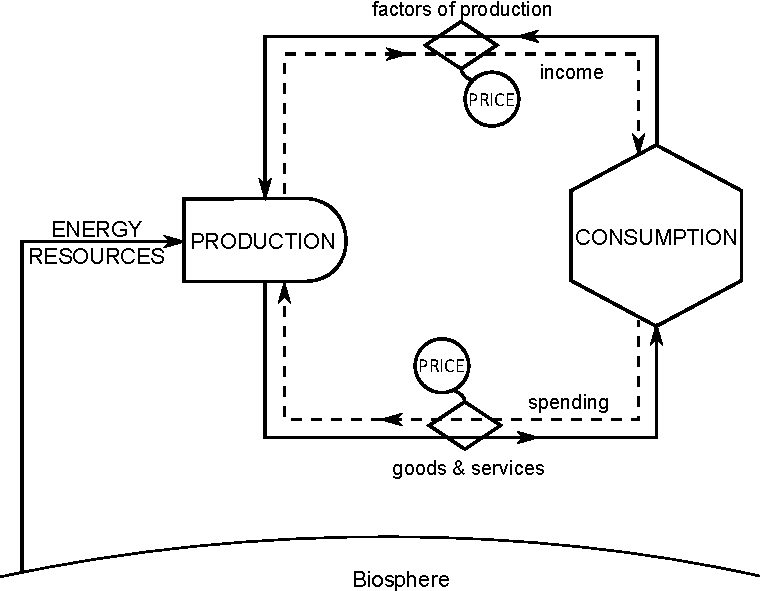
\includegraphics[width=\linewidth]{Part_0/Chapter_Introduction/images/Perpetual_motion_2.pdf}
\caption[The traditional model supplemented with resource inputs]{Energy 
and material input output analysis has included the flows into the economy from the environment.
This may be considered a perpetual motion machine 
of the second kind.
[SHOULD FLOW FROM `RAW RESOURCES' ALSO GO STRAIGHT INTO CONSUMPTION?]}
\label{fig:perp_motion_2}
\end{figure}

%%%%%%%%%% Metabolic	%%%%%%%%%% 
\subsection{The metabolic economy}
\label{sec:metabolic}
%%%%%%%%%% 

\begin{itemize}
	\item{Boulding's ``spaceship Earth''}
\end{itemize}

Review \cite{F-K2003}

\cite{F-K1998}\cite{ConAccount1998}\cite{Giampietro2000}\cite{Daniels2001}\cite{Ayres2002}\cite{Haberl2001}
\cite{Giampietro2013}

\begin{figure}[!ht]
\centering\
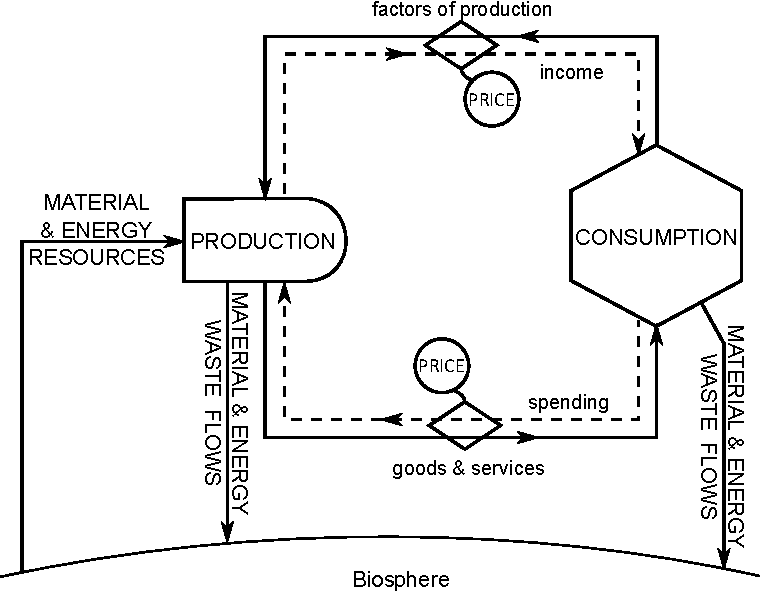
\includegraphics[width=\linewidth]{Part_0/Chapter_Introduction/images/PERKS.pdf}
\caption[A comprehensive biophysical (?) model of the economy]{A comprehensive model 
of the economy, fully consistent with the laws of thermodynamics 
must include degraded resources (waste) expelled 
to the environment as a necessary consequence of economic activity.}
\label{fig:metabolic_economy}
\end{figure}

%%%%%%%%%% I-O History	%%%%%%%%%% 
\section{Brief history of input-output (I-O) modeling}
\label{sec:history}
%%%%%%%%%% 

Input-output analysis, developed by Wassilly Leontief in the 1930s 
as an extension to the work of Quesnay and Walras~\cite{Leontief1936}, 
is of primary importance in national accounting, 
allowing determination of the structure of an economy as well as, 
among other things, 
calculation of a nation's gross domestic product (GDP), 
the predominant measure of economic activity.







%%%%%%%%%% Basic I-O		%%%%%%%%%% 
\subsection{Basic I-O method}
\label{sec:IO_basic}
%%%%%%%%%% 

The basic premise of the I-O method, 
as depicted in Figure~\ref{fig:basic_unit}A, 
is that each economic sector takes in factors of production 
from other sectors (and possibly itself) 
to produce an economic good at some rate. 
For example, the automotive sector takes in steel, rubber, glass, etc. 
and produces a number of cars per year. 
In contrast to high-level economic growth models 
that include only a few factors of production (such as land, capital, and labor), 
the I-O analysis technique allows many differentiated factors of production 
and raw material feedstocks.\cite{Costanza:1980ww} 
In I-O frameworks, each factor of production 
is considered to be a output from a sector of the economy. 
As will be discussed later [MAKE SURE TO DISCUSS THIS LATER!], 
the traditional primary factors of production (land, capital, and labor) 
are not \emph{flows} into the production processes. 
Rather, they are \emph{stocks} that, when present, 
allow factors of production (steel, rubber, and glass) 
to be transformed into final products (automobiles). 
The quantity and quality of these stocks 
determine the quantity and quality of their flow of productive services.

\begin{figure}[!ht]
\centering\
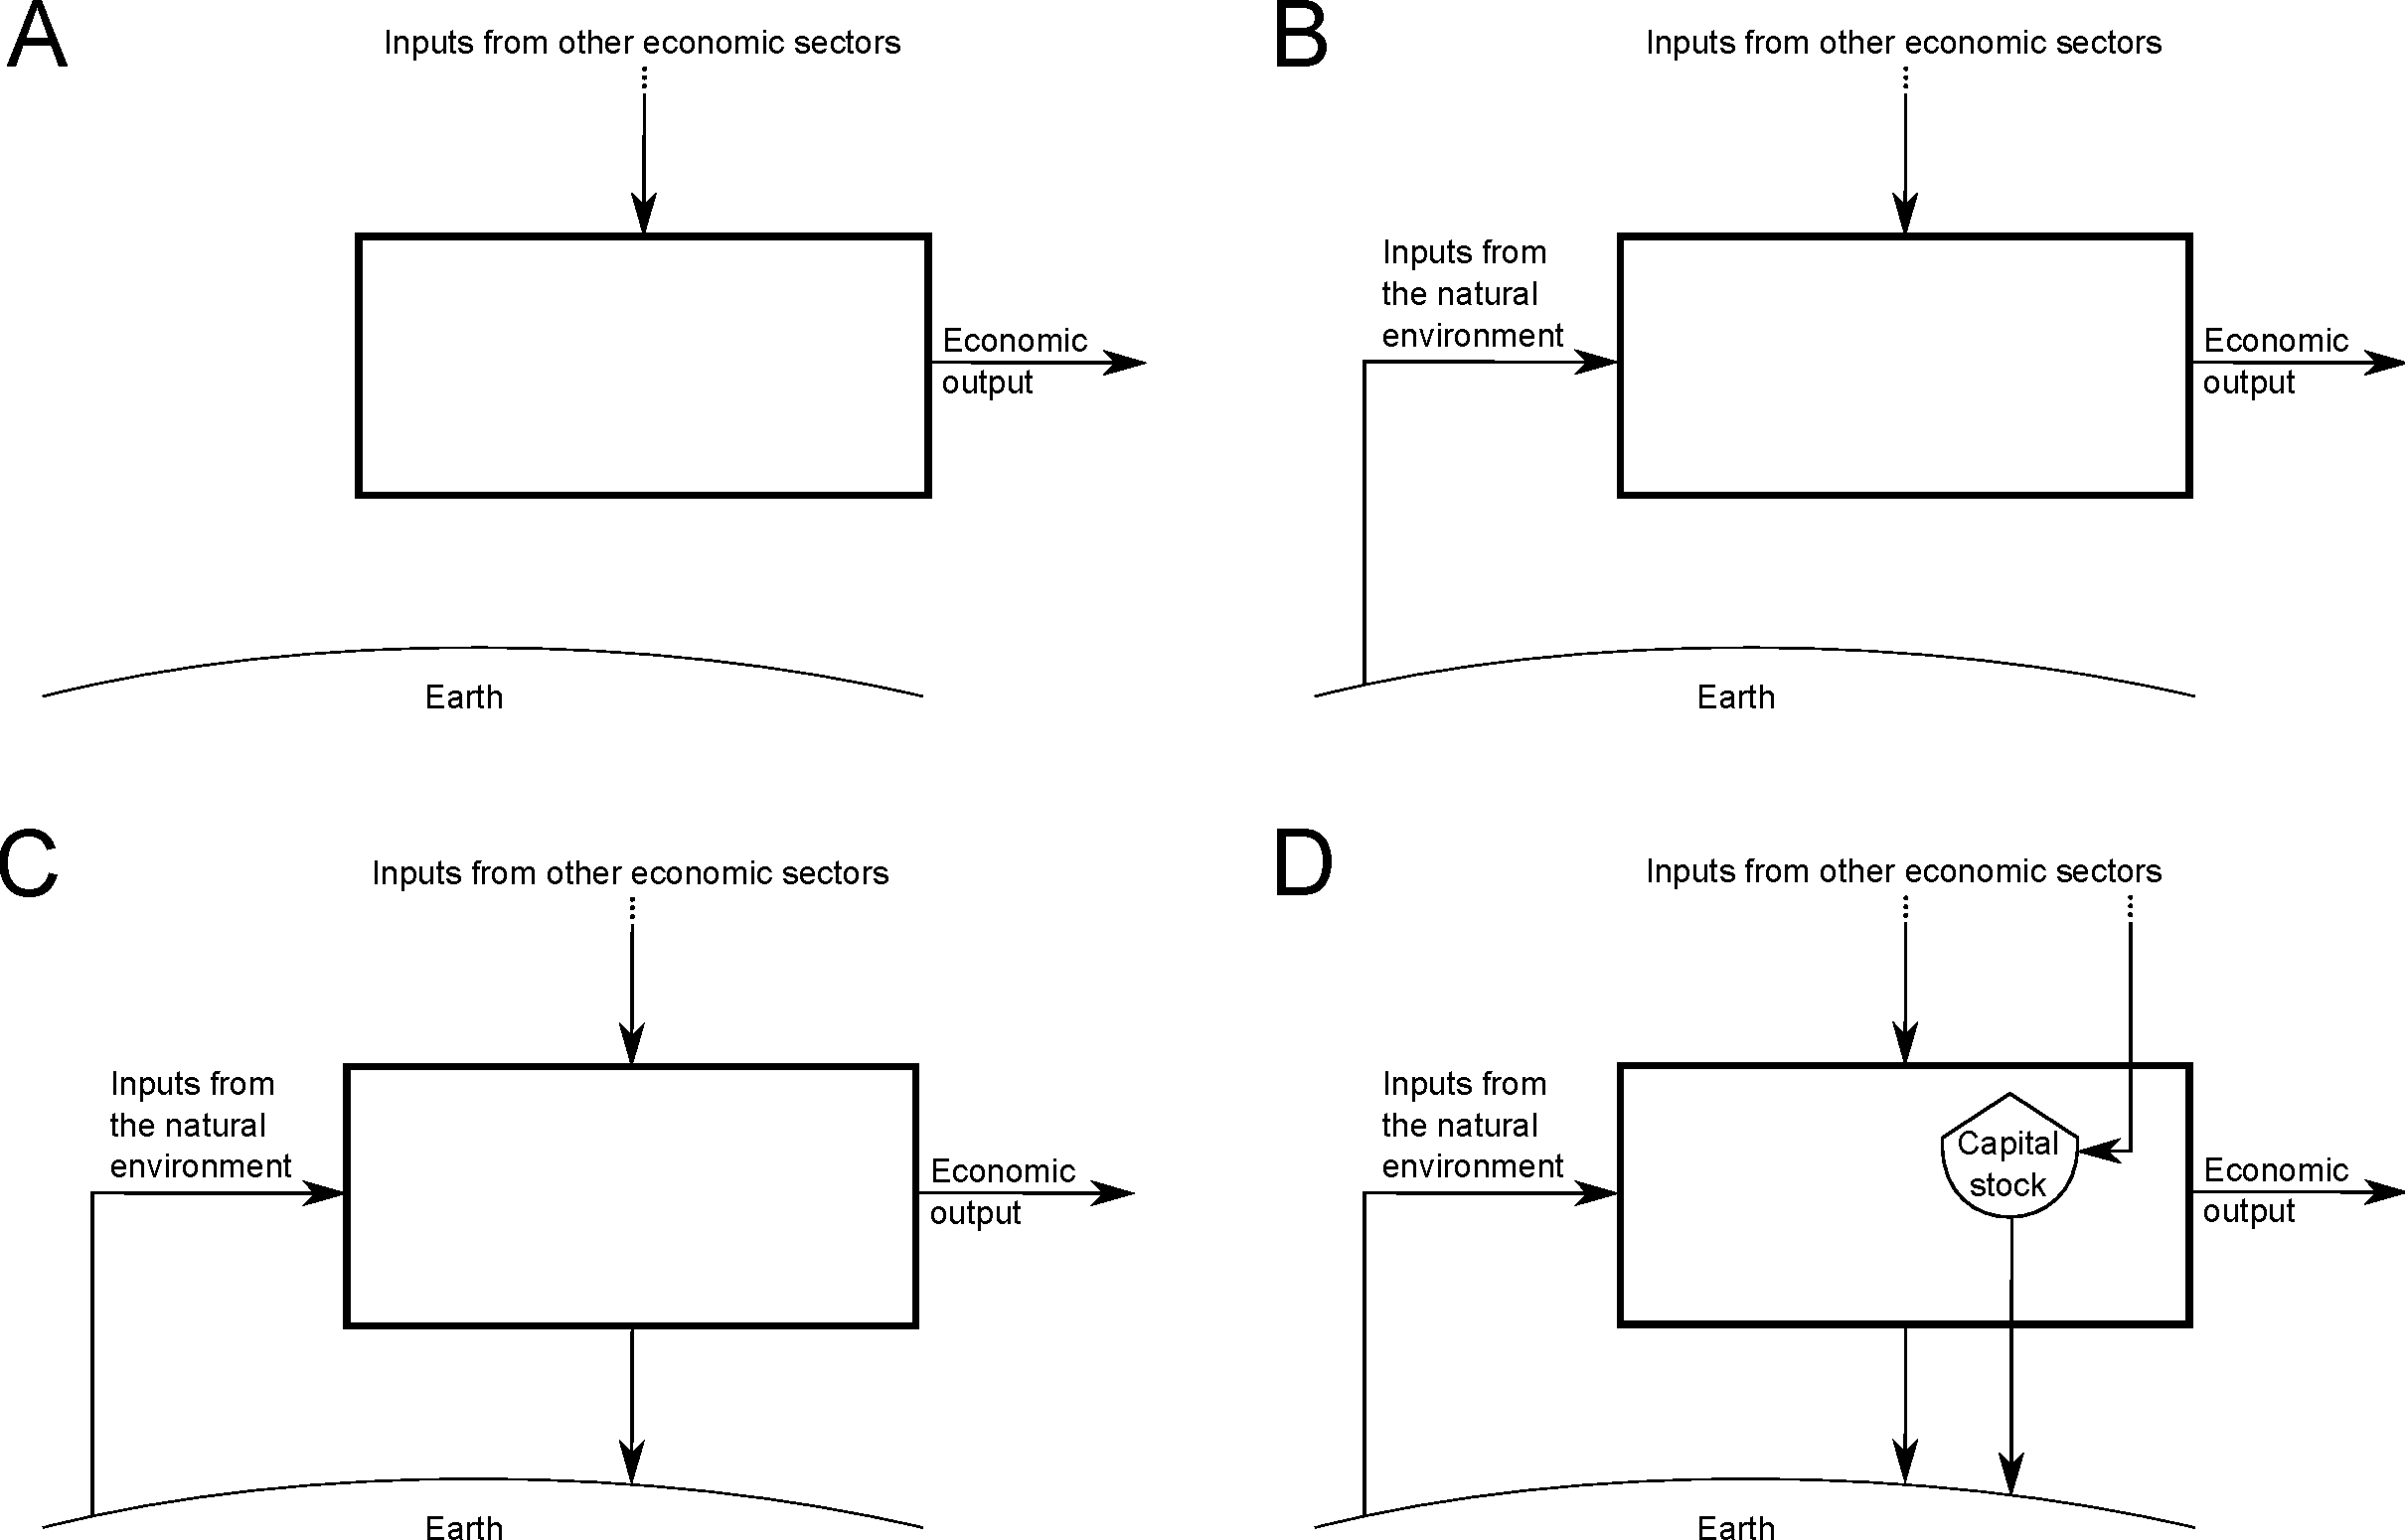
\includegraphics[width=\linewidth]{Part_0/Chapter_Introduction/images/Basic_unit_square.pdf}
\caption[The basic unit of input-output modeling]{The basic unit 
of input-output modeling: 
\textbf{A} the standard economic approach includes only transactions 
among sectors of the economy; 
\textbf{B} the energy input-output approach models inputs 
from the natural environment outside the economy as factors of production; 
\textbf{C} including waste flows to the environment makes the model physically consistent and;
\textbf{D} the method presented here accounts also for accumulation
in capital stock, $K$, of embodied energy within materials in economic sectors. 
[SHOULD WE HAVE THE LABEL ``K'' IN THE ACCUMULATION, OR JUST HAVE THE TANK?]}
\label{fig:basic_unit}
\end{figure}

%%%%%%%%%% Resource I-O	%%%%%%%%%% 
\subsection{I-O method including inputs from the biosphere}
\label{sec:IO_resource}
%%%%%%%%%% 

***** MCD----add this somewhere ****
The making industries related to extraction, refining, and utilities mark the entry point for materials extracted from the biosphere into the economy. These three industries (extraction, refining, and utilities) are the first three industries listed in the NAICS (North American Industry Classification System) that the BEA uses to track economic information. ****BRH add cite (Law- son and et al. 2002, 25). ****

In addition to the productive services provided by stocks of land, capital, and labor,
a flow of energy\footnote{Or, more precisely, 
the degradation of an exergetic gradient/destruction of exergy.} 
is required for economic activity. 
These energy flows originate from the natural environment, 
recognition of which has provoked researchers from fields of 
net energy analysis (NEA), 
material flow analysis (MFA), 
industrial ecology (IE), and 
life-cycle assessment (LCA) 
to extend the traditional (Leontief) input-output framework 
to include important material and energy flows to and from the environment, 
as depicted in Figure~\ref{fig:basic_unit}B.\cite{Carter1974,Bullard1975,Bullard1976a,Herendeen1978,Costanza:1980ww,Casler1984,Joshi:1999uw,Suh2009}
While the Leontief I-O approach relies exclusively 
on monetary units to represent value flows 
among sectors of an economy, 
the key insight of these extensions 
of the Leontief I-O framework is to rely upon physical units 
(especially energy units of joules) 
to represent some of the value flows among economic sectors. 
In doing so, energy and material intensities of value flows can be estimated. 
This extended approach is depicted in Figure~\ref{fig:basic_unit}C. 

Both the original Leontief I-O framework 
and the extensions cited above 
assume steady-state conditions in an economy, 
i.e., flows of value and material into 
and out of each economic sector are in balance. 
Dynamic or transient behavior 
of the economic system is not considered. 
Thus, there is no accumulation of economic factors 
or embodied energy within any of the sectors. 
The analysis techniques provide ``snapshots'' 
of economic activity at an instant in time.

[MIK'S NEW ADDITION]

Assuming no accumulation of materials, 
within economic sectors or society itself, 
is tantamount to assuming that \emph{all} material flows 
through the economy are directed toward the production of non-durable goods. 
However, evidence of the durability of goods 
and the accumulation of materials surrounds us. 
Furthermore, energy was required to both fabricate and emplace 
the durable goods and infrastructure of modern economies. 
(The energy it took to create the durable goods and infrastructure 
can be considered ``embodied'' within the built environment, 
a point to which we will return in detail later). 
As Georgescu-Roegen notes, 
``in the everyday world one cannot possibly cross a river 
only on the flow of maintenance materials of a non-existent bridge.''\cite{G-R1975}

Analysis methods that neglect the accumulation 
of materials and embodied energy 
in the durable goods and infrastructure 
of the everyday world lack explanatory power. 
Such models can tell us at what rates materials and energy are required 
to \emph{use} our built environment. 
But, such models cannot tell us \emph{how} 
the built environment came to be 
(and how much energy was required to construct it) 
or \emph{why} flows of goods are needed. 
To use Georgescu-Roegen's imagery, 
models that neglect accumulation fail to explain 
why we need any material flows to maintain a non-existent bridge. 
Stocks of accumulated materials 
(capital, appliances, even people) 
are the drivers of demand. 
It is to service their needs and wants that we put the economy to work. 

Because economic activity requires energy, 
we need to understand the way energy flows through economies. 
The steady-state I-O techniques of Bullard, Herendeen, 
and others\cite{Bullard1975,Herendeen1978} 
offer a means to that end. 
We contend, however, that these techniques 
need to be extended and modified to include transient effects 
that arise when durability of goods and infrastructure 
(and associated embodied energy) are considered. 
This manuscript attempts to address that need.




%\section{Issues of resource quality}
%
%[DO WE NEED THIS SECTION? IT FEELS LIKE WE SHOULD MOVE FROM THE PREVIOUS SECTION WHEREIN WE CLEARLY DEMONSTRATE THE NEED FOR OUR WORK TO BEGINNING THE PROCESS OF DEVELOPING THE METHOD. IF WE WANT TO KEEP THIS SECTION, WE SHOULD DO A BETTER JOB AT SHOWING WHY IT IS NEEDED. WE SHOULD POINT BACK TO BULLARD AND HERENDEEN AND SAY THAT THEIR METHOD DOESN'T ACCOUNT FOR DECREASING RESOURCE QUALITY AND WHY A METHOD IS NEEDED THAT DOES ACCOUNT FOR DECLINING RESOURCE QUALITY. --MKH] 
% [MCD---I'm going to steal this paragraph for the Unfinished Business chapter.]
%Raw material and energy resources must first be extracted from the natural environment before they may be utilized in the economy to provide goods and service to society. Despite increasing levels of technological efficiency, for example in consumer goods such as refrigerators and cars, evidence shows that the energy intensity of primary resource extraction, i.e. the energy required to extract raw materials from the environment, has been steadily increasing over the last fifty years \cite{Hall1986, Mudd2010, Brandt2011}. This increasing energy requirement for primary extraction means that less \textit{net energy} is available for downstream uses. If this decline in net energy availability outpaces technological advances in energy efficiency, there may be deleterious impacts on the economic output of the economy.

%%%%%%%%%% Waste IO	%%%%%%%%%% 
\subsection{I-O methods including resource inputs and waste flows}
\label{sec:IO_waste}
%%%%%%%%%% 

\cite{Lenzen1998}\cite{ConAccount1998}\cite{Hoekstra2003}\cite{Bailey2008}
\cite{Pedersen2006}\cite{Turner2007}

%%%%%%%%%% Dynamic IO		%%%%%%%%%% 
\subsection{An I-O method for dynamic (transient) economic analysis}
\label{sec:IO_dynamic}
%%%%%%%%%% 

But why do we have consumption?
Boulding tells us that consumption is the 
real cost of living in a physical world.
That there is, ``no particular virtue in consumption. 
It is, unfortunately, 
a necessary incident in the business of living. 
We cannot eat without destroying food; 
we cannot walk without destroying shoes; 
we cannot drive without destroying gasoline, 
tires, and cars; and so on.''\cite[p.2]{Boulding1945}


\begin{itemize}
\item{Boulding (1945)\cite{Boulding1945}, pp.\ 2--3 are fantastic! Consumption is the real cost of living in a physical
	world. Capital cannot accumulate indefinitely.
	When we reach steady state, we must either decrease production (causing unemployment)
	or increase consumption.}
	\item{Important to highlight difference between material depreciation (Boulding's `consumption') and financial depreciation.}
	\item{Financial depreciation is typically (under normal circumstances) a leading indicator of material depreciation}
\end{itemize}

\begin{itemize}
	\item{Daly (2002)\cite{Daly2002}: \emph{efficient} causes (land, capital, labor) vs. \emph{material} causes (resources).
	This is equivalent to GR's needle vs.\ cloth or \emph{flow} vs.\ \emph{fund}.}
		\item{Prior to accumulation, embodied energy is passed into (allocated to) products.}	
	\item{Embodied energy flows with material, not with dollars}
\end{itemize}

In this manuscript, we develop a physical input-output, 
matrix-based method for modeling multi-sector economies, 
in the tradition of Georgescu-Roegen's ``flow-fund'' 
model.\cite{G-R1979a, G-R1979b} 
The method presented in this paper takes a decidedly engineering approach
**** Need to re-cast in metabolism language!!!! **** 
to extend the techniques of Bullard, Herendeen, and others 
to account for durability of goods and embodied energy. 
This method allows us to see how energy and materials flow through the economy, 
where embodied energy accumulates in the economy, 
and how declining resource quality may affect these dynamics. 
[NEED TO MAKE SURE WE ACHIEVE THIS LAST POINT]

%%%%%%%%%% Structure	%%%%%%%%%% 
\section{Organization of this book}
\label{sec:structure}
%%%%%%%%%% 

The remainder of this book is organized as follows. 
Chapter~\ref{chap:materials} presents a discussion of material flows through economies.
Flows of direct energy are discussed in Chapter~\ref{chap:direct_energy}, 
and a rigorous, thermodynamics-based definition of and accounting for 
embodied energy is presented in Chapter~\ref{chap:embodied_energy}. 
Flows of economic value and the energy intensity of economic output are
discussed in Chapters~\ref{chap:value}~and~\ref{chap:intensity}, respectively.
Chapter~\ref{chap:implications} draws some implications 
from the framework for economic growth and other important topics.
Finally, Chapter~\ref{chap:unfinished_business} looks at 
unfinished business: practical, conceptual, and theoretical issues
that arise in the development of this framework.

In Chapters~\ref{chap:materials}--\ref{chap:intensity},
we develop our dynamic framework for materials and energy accounting
through a series of increasingly-disaggregated
models of the economy (Table~\ref{tab:examplesABC}). 
In addition, we use the the US auto industry 
as a running example for application and discussion.

\begin{table}
\caption{Examples
used throughout this book}
\begin{center}
  \begin{tabular}{r @{\hspace{2em}} c @{\hspace{2em}} c @{\hspace{2em}} c @{\hspace{2em}} c}
    \toprule
    Example & Sector 0 & Sector 1 & Sector 2 & Sector 3 \\ 
	\midrule
    A & Biosphere	&	Society            & NA         & NA                 \\
    B & Biosphere	&	Final Consumption  & Production & NA                 \\
    C & Biosphere	&	Final Consumption  & Energy     & Goods \& Services  \\
  \bottomrule
  \end{tabular}
\end{center}
\label{tab:examplesABC}
\end{table}


\bibliographystyle{unsrt}
\bibliography{../../EROI_review_v2}


% Always give a unique label
% and use \ref{<label>} for cross-references
% and \cite{<label>} for bibliographic references
% use \sectionmark{}
% to alter or adjust the section heading in the running head
%% Instead of simply listing headings of different levels we recommend to let every heading be followed by at least a short passage of text. Furtheron please use the \LaTeX\ automatism for all your cross-references and citations.

%% Please note that the first line of text that follows a heading is not indented, whereas the first lines of all sequent paragraphs are.

%% Use the standard \verb|equation| environment to typeset your equations, e.g.
%
%% \begin{equation}
%% a \times b = c\;,
%% \end{equation}
%
%% however, for multiline equations we recommend to use the \verb|eqnarray|
%% environment\footnote{In physics texts please activate the class option \texttt{vecphys} to depict your vectors in \textbf{\itshape boldface-italic} type - as is customary for a wide range of physical jects.}.
%% \begin{eqnarray}
%% a \times b = c \nonumber\\
%% \vec{a} \cdot \vec{b}=\vec{c}
%% \label{eq:01}
%% \end{eqnarray}

%% \section{section Heading}
%% \label{sec:2}
%% Instead of simply listing headings of different levels we recommend to let every heading be followed by at least a short passage of text. Furtheron please use the \LaTeX\ automatism for all your cross-references\index{cross-references} and citations\index{citations} as has already been described in Sect.~\ref{sec:2}.

%% \begin{quotation}
%% Please do not use quotation marks when quoting texts! Simply use the \verb|quotation| environment -- it will automatically render Springer's preferred layout.
%% \end{quotation}


%% \section{section Heading}
%% Instead of simply listing headings of different levels we recommend to let every heading be followed by at least a short passage of text. Furtheron please use the \LaTeX\ automatism for all your cross-references and citations as has already been described in Sect.~\ref{sec:2}, see also Fig.~\ref{fig:1}\footnote{If you copy text passages, figures, or tables from other works, you must obtain \textit{permission} from the copyright holder (usually the original publisher). Please enclose the signed permission with the manucript. The sources\index{permission to print} must be acknowledged either in the captions, as footnotes or in a separate section of the book.}

%% Please note that the first line of text that follows a heading is not indented, whereas the first lines of all sequent paragraphs are.

% For figures use
%
%% \begin{figure}[b]
%% \sidecaption
% Use the relevant command for your figure-insertion program
% to insert the figure file.
% For example, with the option graphics use
%% \includegraphics[scale=.65]{figure}
%
% If not, use
%\picplace{5cm}{2cm} % Give the correct figure height and width in cm
%
%% \caption{If the width of the figure is less than 7.8 cm use the \texttt{sidecapion} command to flush the caption on the left side of the page. If the figure is positioned at the top of the page, align the sidecaption with the top of the figure -- to achieve this you simply need to use the optional argument \texttt{[t]} with the \texttt{sidecaption} command}
%% \label{fig:1}       % Give a unique label
%% \end{figure}


%% \paragraph{Paragraph Heading} %
%% Instead of simply listing headings of different levels we recommend to let every heading be followed by at least a short passage of text. Furtheron please use the \LaTeX\ automatism for all your cross-references and citations as has already been described in Sect.~\ref{sec:2}.

%% Please note that the first line of text that follows a heading is not indented, whereas the first lines of all sequent paragraphs are.

%% For typesetting numbered lists we recommend to use the \verb|enumerate| environment -- it will automatically render Springer's preferred layout.

%% \begin{enumerate}
%% \item{Livelihood and survival mobility are oftentimes coutcomes of uneven socioeconomic development.}
%% \begin{enumerate}
%% \item{Livelihood and survival mobility are oftentimes coutcomes of uneven socioeconomic development.}
%% \item{Livelihood and survival mobility are oftentimes coutcomes of uneven socioeconomic development.}
%% \end{enumerate}
%% \item{Livelihood and survival mobility are oftentimes coutcomes of uneven socioeconomic development.}
%% \end{enumerate}


%% \paragraph{paragraph Heading} In order to avoid simply listing headings of different levels we recommend to let every heading be followed by at least a short passage of text. Use the \LaTeX\ automatism for all your cross-references and citations as has already been described in Sect.~\ref{sec:2}, see also Fig.~\ref{fig:2}.

%% Please note that the first line of text that follows a heading is not indented, whereas the first lines of all sequent paragraphs are.

%% For unnumbered list we recommend to use the \verb|itemize| environment -- it will automatically render Springer's preferred layout.

%% \begin{itemize}
%% \item{Livelihood and survival mobility are oftentimes coutcomes of uneven socioeconomic development, cf. Table~\ref{tab:1}.}
%% \begin{itemize}
%% \item{Livelihood and survival mobility are oftentimes coutcomes of uneven socioeconomic development.}
%% \item{Livelihood and survival mobility are oftentimes coutcomes of uneven socioeconomic development.}
%% \end{itemize}
%% \item{Livelihood and survival mobility are oftentimes coutcomes of uneven socioeconomic development.}
%% \end{itemize}

%% \begin{figure}[t]
%% \sidecaption[t]
% Use the relevant command for your figure-insertion program
% to insert the figure file.
% For example, with the option graphics use
%% \includegraphics[scale=.65]{figure}
%
% If not, use
%\picplace{5cm}{2cm} % Give the correct figure height and width in cm
%
%% \caption{Please write your figure caption here}
%% \label{fig:2}       % Give a unique label
%% \end{figure}

%% \runinhead{Run-in Heading Boldface Version} Use the \LaTeX\ automatism for all your cross-references and citations as has already been described in Sect.~\ref{sec:2}.

%% \runinhead{Run-in Heading Italic Version} Use the \LaTeX\ automatism for all your cross-refer\-ences and citations as has already been described in Sect.~\ref{sec:2}\index{paragraph}.
% Use the \index{} command to code your index words
%
% For tables use
%
%% \begin{table}
%% \caption{Please write your table caption here}
%% \label{tab:1}       % Give a unique label
%
% For LaTeX tables use
%
%% \begin{tabular}{p{2cm}p{2.4cm}p{2cm}p{4.9cm}}
%% \hline\noalign{\smallskip}
%% Classes & class & Length & Action Mechanism  \\
%% \noalign{\smallskip}\svhline\noalign{\smallskip}
%% Translation & mRNA$^a$  & 22 (19--25) & Translation repression, mRNA cleavage\\
%% Translation & mRNA cleavage & 21 & mRNA cleavage\\
%% Translation & mRNA  & 21--22 & mRNA cleavage\\
%%Translation & mRNA  & 24--26 & Histone and DNA Modification\\
%%\noalign{\smallskip}\hline\noalign{\smallskip}
%%\end{tabular}
%%$^a$ Table foot note (with superscript)
%%\end{table}
%
%% \section{Section Heading}
%%\label{sec:3}
% Always give a unique label
% and use \ref{<label>} for cross-references
% and \cite{<label>} for bibliographic references
% use \sectionmark{}
% to alter or adjust the section heading in the running head
%% Instead of simply listing headings of different levels we recommend to let every heading be followed by at least a short passage of text. Furtheron please use the \LaTeX\ automatism for all your cross-references and citations as has already been described in Sect.~\ref{sec:2}.

%% Please note that the first line of text that follows a heading is not indented, whereas the first lines of all sequent paragraphs are.

%%If you want to list definitions or the like we recommend to use the Springer-enhanced \verb|description| environment -- it will automatically render Springer's preferred layout.

%%\begin{description}[Type 1]
%%\item[Type 1]{That addresses central themes pertainng to migration, health, and disease. In Sect.~\ref{sec:1}, Wilson discusses the role of human migration in infectious disease distributions and patterns.}
%%\item[Type 2]{That addresses central themes pertainng to migration, health, and disease. In Sect.~\ref{sec:2}, Wilson discusses the role of human migration in infectious disease distributions and patterns.}
%%\end{description}

%%\section{section Heading} %
%% In order to avoid simply listing headings of different levels we recommend to let every heading be followed by at least a short passage of text. Use the \LaTeX\ automatism for all your cross-references and citations citations as has already been described in Sect.~\ref{sec:2}.

%% Please note that the first line of text that follows a heading is not indented, whereas the first lines of all sequent paragraphs are.

%% \begin{svgraybox}
%% If you want to emphasize complete paragraphs of texts we recommend to use the newly defined Springer class option \verb|graybox| and the newly defined environment \verb|svgraybox|. This will produce a 15 percent screened box 'behind' your text.

%% If you want to emphasize complete paragraphs of texts we recommend to use the newly defined Springer class option and environment \verb|svgraybox|. This will produce a 15 percent screened box 'behind' your text.
%% \end{svgraybox}


%% \section{section Heading}
%%Instead of simply listing headings of different levels we recommend to let every heading be followed by at least a short passage of text. Furtheron please use the \LaTeX\ automatism for all your cross-references and citations as has already been described in Sect.~\ref{sec:2}.

%% Please note that the first line of text that follows a heading is not indented, whereas the first lines of all sequent paragraphs are.

%% \begin{theorem}
%% Theorem text goes here.
%% \end{theorem}
%
% or
%
%% \begin{definition}
%% Definition text goes here.
%% \end{definition}

%% \begin{proof}
%\smartqed
%% Proof text goes here.
%% \qed
%% \end{proof}

%%\paragraph{Paragraph Heading} %
%% Instead of simply listing headings of different levels we recommend to let every heading be followed by at least a short passage of text. Furtheron please use the \LaTeX\ automatism for all your cross-references and citations as has already been described in Sect.~\ref{sec:2}.

%% Note that the first line of text that follows a heading is not indented, whereas the first lines of all subsequent paragraphs are.
%
% For built-in environments use
%
%%\begin{theorem}
%%Theorem text goes here.
%%\end{theorem}
%
%%\begin{definition}
%%Definition text goes here.
%%\end{definition}
%
%%\begin{proof}
%%\smartqed
%% Proof text goes here.
%%\qed
%%\end{proof}
%
%% \begin{acknowledgement}
%% If you want to include acknowledgments of assistance and the like at the end of an individual chapter please use the \verb|acknowledgement| environment -- it will automatically render Springer's preferred layout.
%% \end{acknowledgement}
%
%% \section*{Appendix}
%% \addcontentsline{toc}{section}{Appendix}
%
%% When placed at the end of a chapter or contribution (as opposed to at the end of the book), the numbering of tables, figures, and equations in the appendix section continues on from that in the main text. Hence please \textit{do not} use the \verb|appendix| command when writing an appendix at the end of your chapter or contribution. If there is only one the appendix is designated ``Appendix'', or ``Appendix 1'', or ``Appendix 2'', etc. if there is more than one.

%% \begin{equation}
%% a \times b = c
%% \end{equation}
% Problems or Exercises should be sorted chapterwise
%% \section*{Problems}
%% \addcontentsline{toc}{section}{Problems}
%
% Use the following environment.
% Don't forget to label each problem;
% the label is needed for the solutions' environment
%% \begin{prob}
%% \label{prob1}
%% A given problem or Excercise is described here. The
%% problem is described here. The problem is described here.
%% \end{prob}

%% \begin{prob}
%% \label{prob2}
%% \textbf{Problem Heading}\\
%% (a) The first part of the problem is described here.\\
%% (b) The second part of the problem is described here.
%% \end{prob}


